\section{ Fundamentals of Motion: Skipping Re-Entry }\label{sec:q4}    
\subsection*{a.}
\begin{equation}
    \begin{split}
        m \frac{dV}{dt} = -D - mg\sin{(\gamma)} \\
        m V \frac{d \gamma}{dt} = L - mg \cos{(\gamma)}(1-\frac{V^2}{V_c^2}) \\
        \frac{dr}{dt} = \frac{dh}{dt} = V\sin{(\gamma)}
    \end{split}
\end{equation}

For skipping flight, we have that the weight is much smaller than the lift and the drag. Thus, we can approximate the above equations with:

\begin{equation}
    \begin{split}
        m \frac{dV}{dt} = -D  \\
        m V \frac{d \gamma}{dt} = L  \\
        \frac{dr}{dt} = \frac{dh}{dt} = V\sin{\gamma}
    \end{split}
\end{equation}

Now divide the first equation by the second to obtain:

\begin{equation}
    \frac{\frac{dV}{dt}}{V \frac{d \gamma }{dt}} = -\frac{D}{L}
\end{equation}

This gives then:

\begin{equation}
    \frac{dV}{d \gamma}  = - V \frac{D}{L}
\end{equation}

Or, alternatively:

\begin{equation}
    \frac{1}{V} dV = - \frac{D}{L} d\gamma
\end{equation}

Integration gives then:
\begin{equation}
    \begin{split}
        \int_{V_E}^V \frac{1}{V} dV = \int_{\gamma_E}^{\gamma} - \frac{D}{L} d\gamma \\
        \ln{(\frac{V}{V_E})} =  - \frac{D}{L}(\gamma - \gamma_E)  \\
        \frac{V}{V_E} =  \exp{(- \frac{(\gamma - \gamma_E)}{\frac{L}{D}})}  \\
    \end{split}
\end{equation}

For the latter, we have:

\begin{equation}
    V \frac{d \gamma}{dt} = V \frac{\partial \gamma}{\partial p} \frac{\partial p}{\partial h} \frac{\partial h}{\partial t}  = \frac{L}{m}
\end{equation}

This then leads to:

\begin{equation}
\begin{split}
     \frac{\partial p}{\partial t} = \frac{L}{m V} \frac{\partial p}{\partial \gamma} \\ 
    \frac{-L}{\rho g m V} \frac{\partial p}{\partial \gamma} = V \sin{(\gamma)}
\end{split}
\end{equation}
This was done via $\frac{dh}{dt} = V\sin{(\gamma)}$ and $\frac{d p}{d h} = -\rho g$.

We then get:
\begin{equation}
\begin{split}
     \sin{(\gamma)}d\gamma = - \frac{L}{\rho g m} \frac{1}{V^2} dp \\
     \sin{(\gamma)}d\gamma = - \frac{\frac{1}{2}\rho C_L V^2 S}{\rho g m} \frac{1}{V^2} dp \\
     \sin{(\gamma)}d\gamma = - \frac{\rho C_L S}{2 W} dp \\
\end{split}
\end{equation}

Integration then gives:

\begin{equation}
    \begin{split}
        \int_{\gamma_E}^{\gamma} \sin{(\gamma)}d\gamma = \int_{p_E}^p - \frac{\rho C_L S}{2 W} dp \\
        \cos{(\gamma - \gamma_E)}d\gamma =  \frac{\rho C_L S}{2 W} (p-p_E) \\
    \end{split}
\end{equation}

Note that due to the ideal gas law, $p-p_E = \frac{g}{\beta} (\rho - \rho_E)$. Also, on the top of the atmosphere $\rho_E \approx 0$. Together, this finally gives:

\begin{equation}
    \cos{(\gamma)} - \cos{(\gamma_E)} =  \frac{g}{2 \beta} \frac{1}{\frac{W/S}{C_L}} \rho 
\end{equation}

\subsection*{b.}

On the lowest point of the first skipping trajectory, we have that $\frac{d h}{dt} = 0 = V \sin{(\gamma)}$ and thus that $\gamma = 0$. Then we have:
\begin{equation}
\begin{split}
    V = V_E \cdot \exp{(- \frac{(\gamma - \gamma_E)}{\frac{L}{D}})}\\
    V = 8000 \cdot \exp{-\frac{(0 - -0.262 rad)}{1}} = 6157 m/s\\
    \end{split}
\end{equation}

For the exit angle of the first skipping trajectory, we have $\rho \approx 0$, thus $\cos{(\gamma) - \cos{(\gamma_E)}} = 0$, leading to $\gamma = -\gamma_E$. This gives for V:

\begin{equation}
    \begin{split}
    V = V_E \cdot \exp{(- \frac{(\gamma - \gamma_E)}{\frac{L}{D}})}\\
    V_{F,1} = 8000 \cdot \exp{-\frac{(0.262 - -0.262 rad)}{1}} = 4737 m/s\\
    \end{split}
\end{equation}

For the top of the ballistic flight after the first skipping trajectory, we have that the vertical velocity is zero and the horizontal velocity is equal to that when the atmosphere was left, thus $V_h = V_{F,1} \cos{(\gamma_{F,1})} = 4737 \cdot 0.966 = 4576 m/s$. Of course, on the top also $\gamma = 0$.

For the next point, we assume that above the atmosphere no friction occurs and thus that the force field is conservative. Then $\gamma_{E,2} = - \gamma_{F,1} = - 15^o$ and $V_{E,2} = V_{F,1} = 4737 m/s$.

For the lowest point of the second skipping trajectory and the exit of the atmosphere of the second skipping trajectory, equal considerations hold and analogously, we obtain $\gamma = 0$ and $V = 3645 m/s$ for the lowest part of the second skip and $\gamma_{F,2} = 15^o$, $V_{F,2} = 2805 m/s$ for the exit of the atmosphere at the end of the second skipping trajectory.

The resulting graph can be seen underneath:

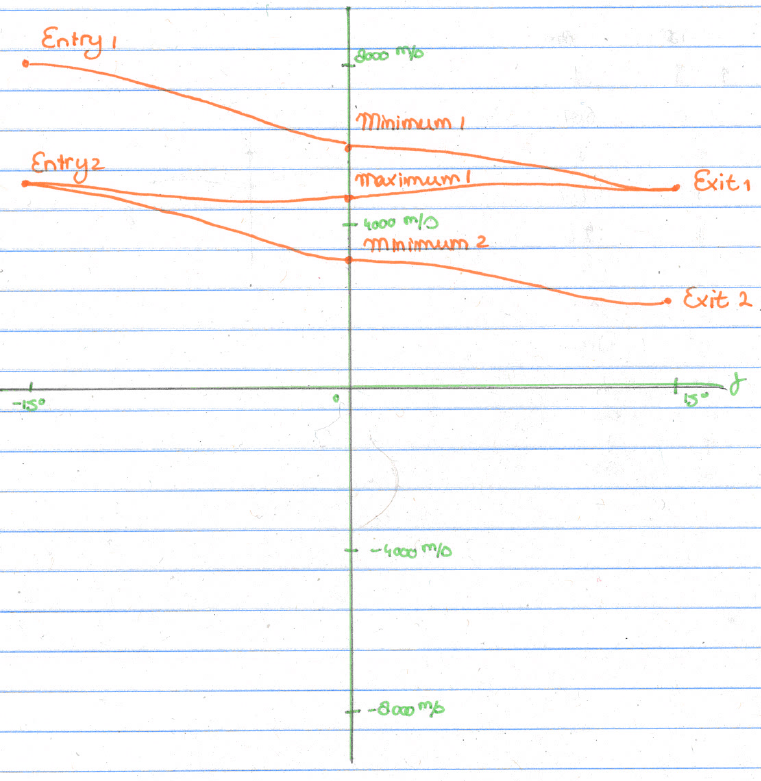
\includegraphics[scale = 1]{SkippingFlight.PNG}

\subsection*{c}
In the lowest point, we have that $\frac{dh}{dt} = 0 = V \sin{(\gamma)}$, thus that $\gamma =0$. Then 

\begin{equation}
        1 - \cos{(\gamma_E)} =  \frac{g}{2 \beta} \frac{1}{\frac{W/S}{C_L}} \rho 
\end{equation}

Using $\sin{(\gamma_E/2)}^2 = 1/2 - 1/2 \cos{(\gamma_E)}$, we get then:

\begin{equation}
    \begin{split}
        \rho_p = 2 \sin{(\gamma_E/2)}^2 \frac{2 \beta}{g} \frac{W/S}{C_L} \\
        \rho_p = \sin{(\gamma_E/2)}^2 \frac{4 \beta}{g} \frac{W/S}{C_L} \\
    \end{split}
\end{equation}

As can be seen, this is independent of the entrance velocity. Now since 
\begin{equation}
    \rho = \rho_0 \exp{(-\beta h)} = \rho_0 \exp{(-\frac{ h}{H})}
\end{equation}

We get:

\begin{equation}
    h_p = -H \ln{(\frac{\rho_p}{\rho_0})}
\end{equation}

Now $\rho_p = 0.0078 kg/m^3$ for both lowest points of the dual skipping entry. This then leads to a value of $h_p = 35392 m$ for both lowest points of the dual skipping entry. 

